\section{Domain Model}
To build an agent that can play poker, the agent has to be able to choose one of the three legal actions: \textit{Fold}, \textit{Call}, or \textit{Raise}. For the raise action, the bot needs to choose also a raise amount, which has to be greater than the highest current bet.
While it is possible to treat all game stages the same, we found it reasonable to split the domain into two main compound tasks. The first is responsible for the preflop stage, and the second for the post-flop stages.

\begin{figure}[h]
    \centering
    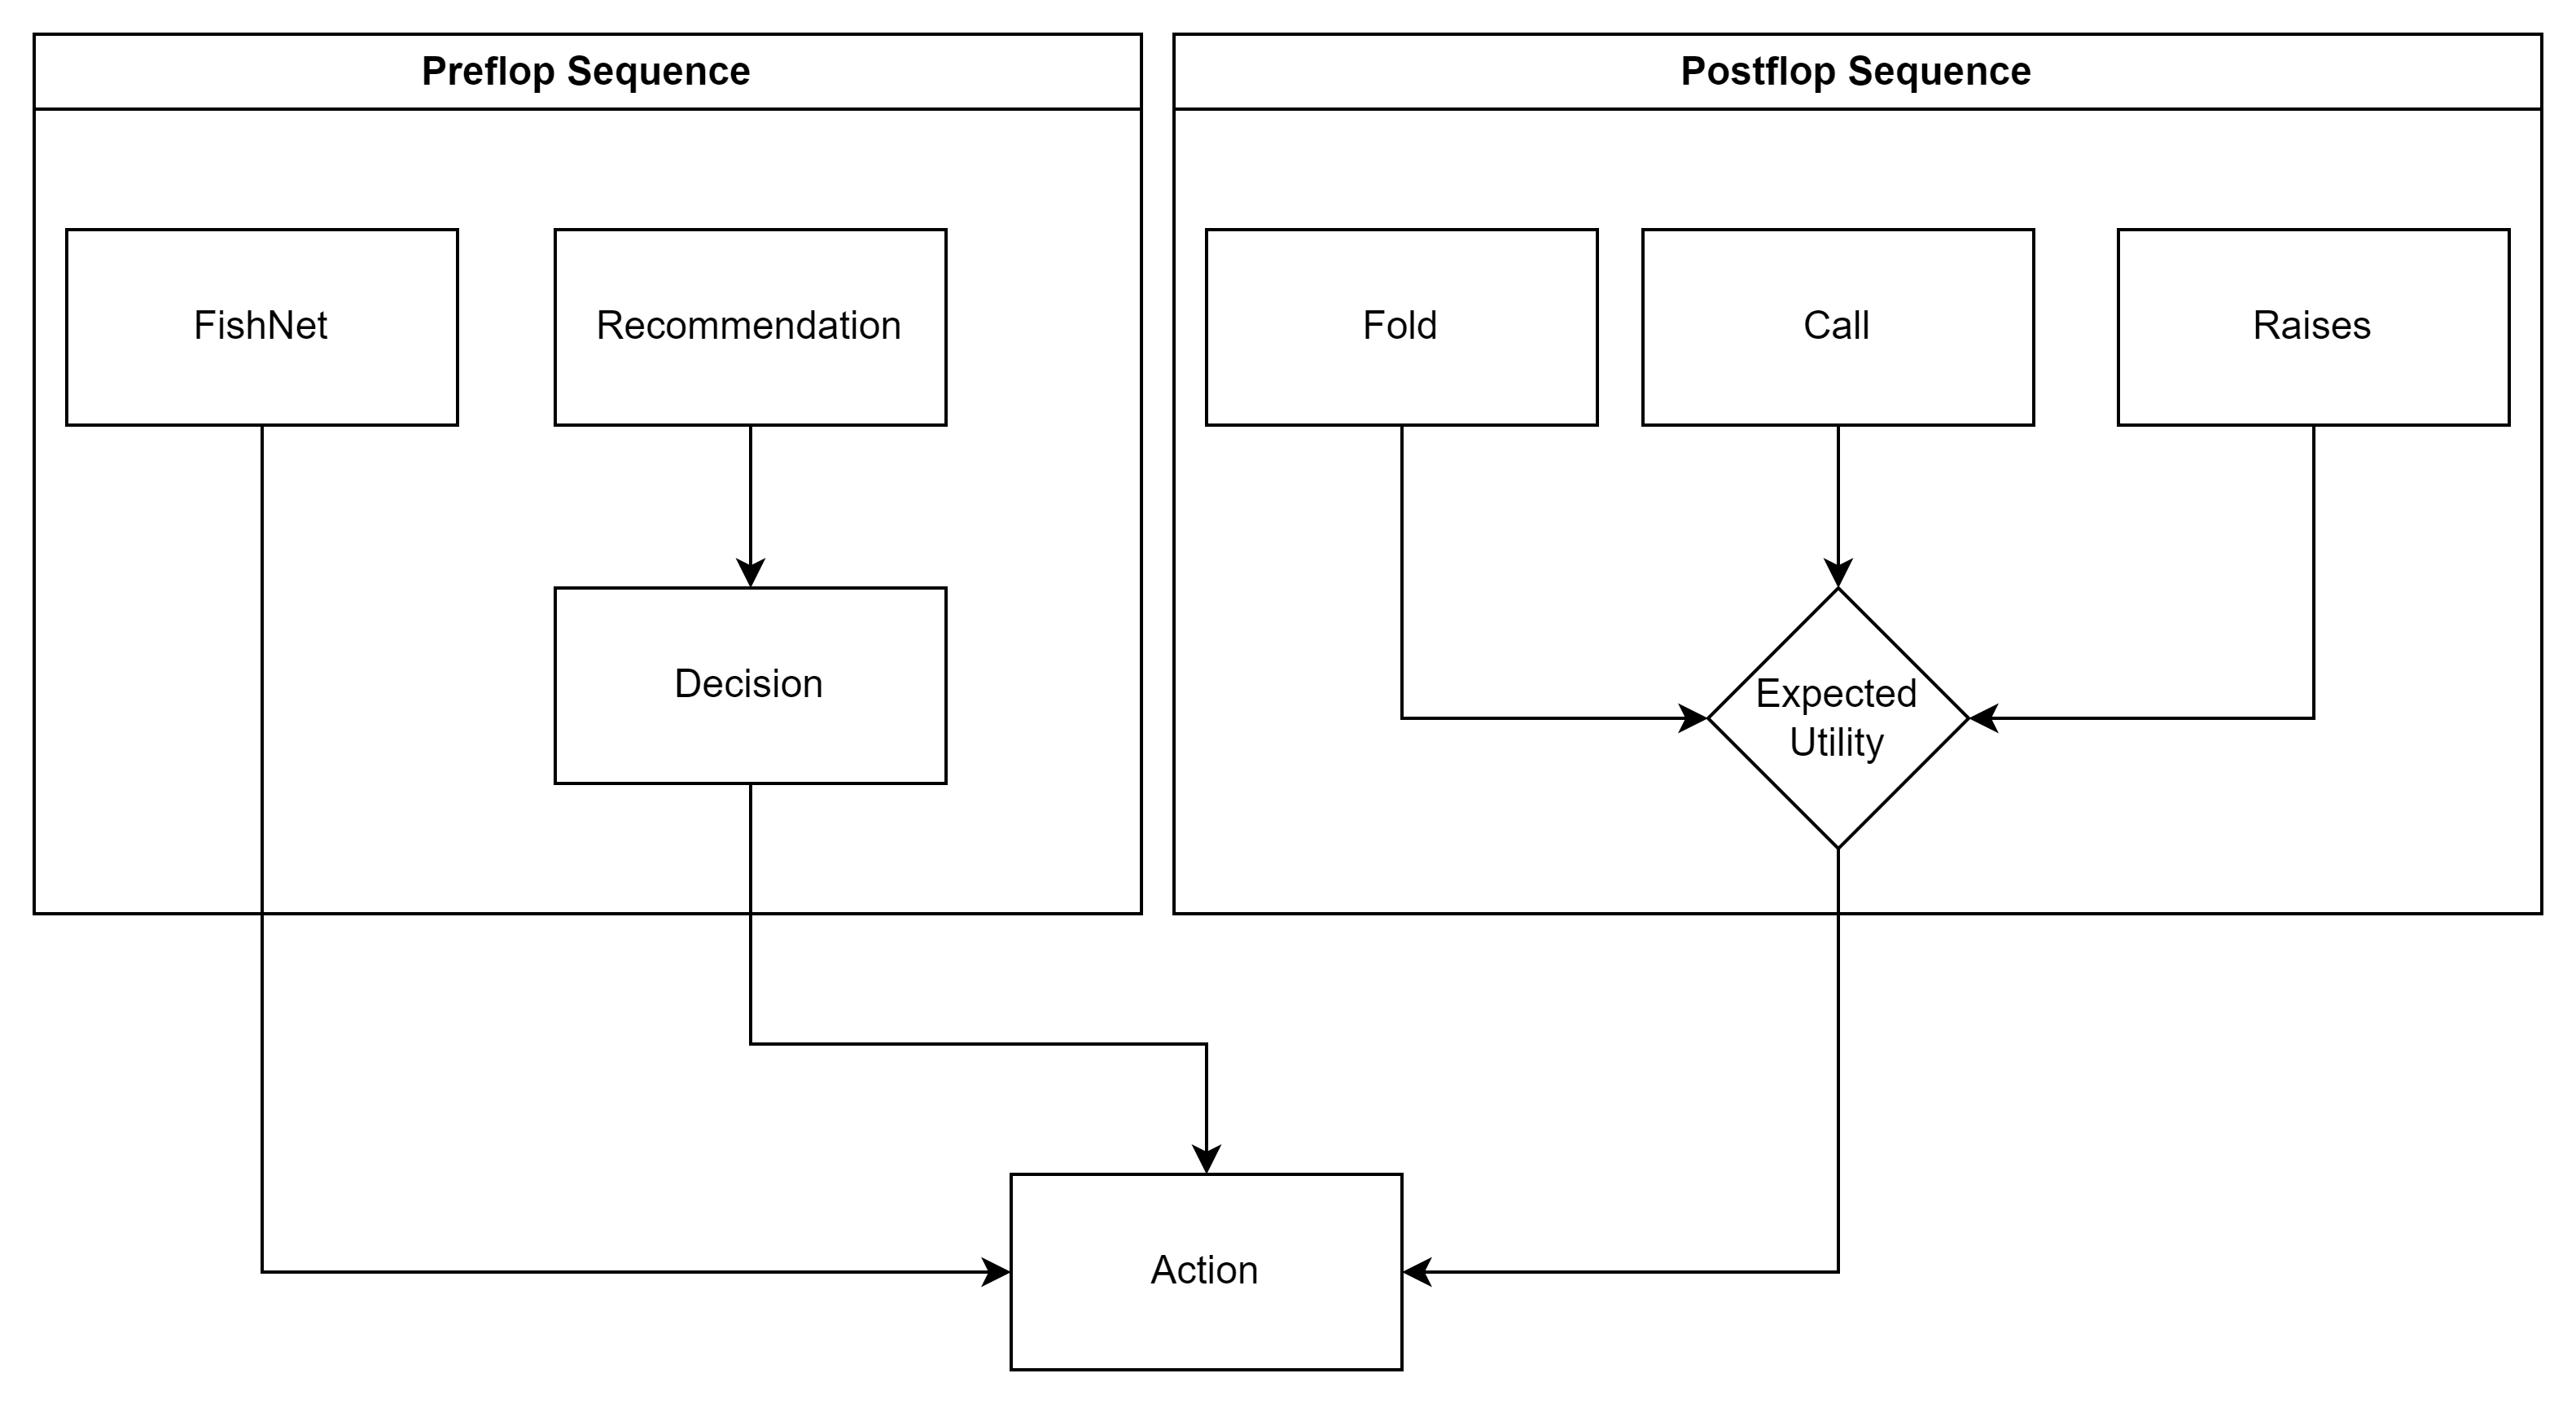
\includegraphics[width=0.9\textwidth]{domain.png}
    \caption{Overview of PokerShark domain model.}
    \label{fig:model}
\end{figure}

The \textit{Preflop Sequence} represents the task responsible for the preflop stage. The sequence includes three compound tasks. The first two tasks will produce a recommendation and convert it to a decision, as described in section 3.3. The last task represents the \textit{Fish Net} discussed in section 3.3.4. The tasks responsible for producing a recommendation are grouped into four compound tasks based on the current position of PokerShark on the table, which is how the original guidelines were grouped in the first place. Each one of these tasks includes a number of compound and primitive tasks representing each guideline. The planner will choose which task to decompose based on a set of preconditions defined for each task. Appendix \ref{appendix:pokerSharkPreconditions} includes a listing of all preconditions used by PokerShark. The \textit{Preflop Sequence} does not use utility or expected utility in the decision-making process. However, the current risk attitude of the agent plays an important role in converting the recommendation into a decision, as described in section 3.3.2.

The \textit{Postflop Sequence} is dynamically generated each time PokerShark is asked to make a decision. The sequence includes one compound task of the custom type \textit{ExpectedUtilitySelector}, meaning this part of the domain is risk aware. For each possible action: Fold, Call and Raise with different bet sizes ranging from the current highest bet to the amount of the current stack, a primitive task of type \textit{VariableUtilityTask} is created. Each one of these tasks gets a utility score assigned based on the current calling amount, money paid, and hand strength. This score is adjusted using the utility function corresponding with the current risk attitude of the agent. The utility score of raise actions is also adjusted based on the amount of the raise and the strength of the hand to ensure that the agent prefers a higher raise amount when it has a stronger hand.

The \textit{FindBestTask} from section 3.4.7 is then used to choose the task with the highest utility. The result of decomposing the best task will be a decision vector. To ensure that the agent will often adopt a slow-playing strategy, the weights in the decision vectors of all raise actions are skewed to prefer calls over raises in the early stages of the round and the other way around in the later stages. 


\section{World State}
The world state of PokerShark is a hash map that contains different objects, such as game and decision objects, in addition to different primitive variables and flags, such as the raise amount and the check-raise flag. It also contains a list of the current legal actions.

The game object is a complex object that contains all the information related to the game, such as the game rules, the number of players, the initial stack, the size of the ante and the blinds, and other related information. It also includes all rounds and action history, including player-related information such as name, stack size, position on the table, and the player model. Nevertheless, the game object and PokerShark have no access to the opponent's current hand; the game server handles this information, and the agent has no access to it.
With each new event, the game server will send a notification to PokerShark, which will update the local game object with the new game state. This allows PokerShark also to update the opponent model after each action performed by the opponent.

The other objects in the world state are used to store information during the planning process. For example, the check-raise flag is used while performing the check-raise tactic, which continues throughout the duration of two stages.


\section{Goal State}
The way PokerShark is set up allows us to run the planner without the need to define a goal state. Instead, we run the planner inside a loop until a flag is set in the world state, which informs us that the planner has decided on an action. The planner requires theoretically only one iteration to reach a decision in the post-flop stage and two iterations in the preflop stage, one to find a recommendation and another to convert it into a decision. Running the planner inside a loop can be problematic, as it can lead to an infinite loop if the agent is in a situation where it cannot make a decision. To solve this problem, we have implemented a timeout mechanism that will stop the planner after a certain number of iterations. If the planner has not found a solution by then, the agent will Fold. 